% AMUN Wind Paper, based on:
% mnras_template.tex
%
% LaTeX template for creating an MNRAS paper
%
% v3.0 released 14 May 2015
% (version numbers match those of mnras.cls)
%
% Copyright (C) Royal Astronomical Society 2015
% Authors:
% Keith T. Smith (Royal Astronomical Society)

% Change log
%
% v3.0 May 2015
%    Renamed to match the new package name
%    Version number matches mnras.cls
%    A few minor tweaks to wording
% v1.0 September 2013
%    Beta testing only - never publicly released
%    First version: a simple (ish) template for creating an MNRAS paper

%%%%%%%%%%%%%%%%%%%%%%%%%%%%%%%%%%%%%%%%%%%%%%%%%%
% Basic setup. Most papers should leave these options alone.
\documentclass[a4paper,fleqn,usenatbib]{mnras}

% MNRAS is set in Times font. If you don't have this installed (most LaTeX
% installations will be fine) or prefer the old Computer Modern fonts, comment
% out the following line
\usepackage{newtxtext,newtxmath}
\usepackage{makecell}
% Depending on your LaTeX fonts installation, you might get better results with one of these:
%\usepackage{mathptmx}
%\usepackage{txfonts}

% Use vector fonts, so it zooms properly in on-screen viewing software
% Don't change these lines unless you know what you are doing
\usepackage[T1]{fontenc}
\usepackage{ae,aecompl}


%%%%% AUTHORS - PLACE YOUR OWN PACKAGES HERE %%%%%

% Only include extra packages if you really need them. Common packages are:
\usepackage{graphicx}	% Including figure files
\usepackage{amsmath}	% Advanced maths commands
\usepackage{amssymb}	% Extra maths symbols
\usepackage{amsfonts}
\usepackage{hyperref}
\usepackage{pifont}

%%%%%%%%%%%%%%%%%%%%%%%%%%%%%%%%%%%%%%%%%%%%%%%%%%

%%%%% AUTHORS - PLACE YOUR OWN COMMANDS HERE %%%%%

% Please keep new commands to a minimum, and use \newcommand not \def to avoid
% overwriting existing commands. Example:
%\newcommand{\pcm}{\,cm$^{-2}$}	% per cm-squared
\usepackage{abbrevs}
\usepackage{xspace}

% FORCE ROMAN FONTS IN SUBSCRIPTS
\begingroup
\catcode`\_=\active
\gdef_#1{\ensuremath{\sb{\mathrm{#1}}}}
\endgroup
\mathcode`\_=\string"8000
\catcode`\_=12


% Revision
% \newcommand{\rev}{\textcolor{Plum}}
\newcommand{\rev}{\textcolor{Black}}

% Useful abbreviations
\newcommand{\Msolar}{M$_{\odot}$\xspace}
\newcommand{\Msolarpc}{M$_{\odot}$ / pc$^{2}$\xspace}
\newcommand{\Zsolar}{Z$_{\odot\xspace}$\xspace}
\newcommand{\Rsolar}{R$_{\odot\xspace}$\xspace}
\newcommand{\Subvir}{$_{vir}$\xspace}
%\newcommand{\atcc}{atoms/cm$^{3}$\xspace}
\newcommand{\atcc}{cm$^{-3}$\xspace}
\newcommand{\mhcc}{m$_{H}$.cm$^{-3}$\xspace}
\newcommand{\simname}{\textsc}
\newcommand{\Stromgren}{Str\"{o}mgren\xspace}
\newcommand{\starsub}{$_{\normalfont\textsc{stars}}$\xspace}
\newcommand{\stars}{\textsc{stars}\xspace}
\newcommand{\turbsub}{$_{\normalfont\textsc{turb}}$\xspace}
\newcommand{\turb}{\textsc{turb}\xspace}
\newcommand{\rcoeff}{$\rho_{X,SFE}$}
\newcommand{\AMUN}{\textsc{amun}}
\newcommand{\HII}{H \textsc{ii}\xspace}

% Graphical commands
%\newcommand{\tick}{$\checkmark$}
\newcommand{\tick}{\hspace{1pt}\ding{51}}
\newcommand{\cross}{\hspace{1pt}\ding{55}}

% Abbreviations
\newabbrev\ISM{Interstellar Medium (ISM)}[ISM]
\newabbrev\CSM{Circumstellar Medium (CSM)}[CSM]
\newabbrev\WNM{Warm Neutral Medium (WNM)}[WNM]
\newabbrev\WIM{Warm Ionised Medium (WIM)}[WIM]
\newabbrev\CNM{Cold Neutral Medium (CNM)}[CNM]
\newabbrev\IMF{Initial Mass Function (IMF)}[IMF]
\newabbrev\CMF{Core Mass Function (IMF)}[IMF]
\newabbrev\AMR{Adaptive Mesh Refinement (AMR)}[AMR]
\newabbrev\HGB{Horizontal Giant Branch (HGB)}[HGB]
\newabbrev\SFE{Star Formation Efficiency (SFE)}[SFE]
\newabbrev\TSFE{Total Star Formation Efficiency (TSFE)}[TSFE]
\newabbrev\OSFE{Observed Star Formation Efficiency (OSFE)}[OSFE]
\newabbrev\SFR{Star Formation Rate (SFR)}[SFR]
\newabbrev\YSOs{Young Stellar Objects (YSOs)}[YSOs]
\newabbrev\YSO{Young Stellar Object (YSO)}[YSO]
\newabbrev\PDF{Probability Distribution Function}[PDF]
\newabbrev\PSF{Point Spread Function}[PSF]
\newabbrev\LMC{Large Magellanic Cloud}[LMC]

% Table gunk
\renewcommand\theadalign{bc}
\renewcommand\theadfont{\bfseries}

\makeatletter
\newcommand*\bigcdot{\mathpalette\bigcdot@{.5}}
\newcommand*\bigcdot@[2]{\mathbin{\vcenter{\hbox{\scalebox{#2}{$\m@th#1\bullet$}}}}}
\makeatother

% Some gumf that makes spaces work properly because abbrevs is buggy: 
% See: http://tex.stackexchange.com/questions/59840/how-to-prevent-getting-a-space-after-an-abbreviation-using-the-abbrevs-package
\makeatletter
\renewcommand\maybe@space@{%
	% \@tempswatrue % <= this is in the original
	\maybe@ictrue % <= this is new
	\expandafter   \@tfor
	\expandafter \reserved@a
	\expandafter :%
	\expandafter =%
	\nospacelist
	\do \t@st@ic
	% \if@tempswa % <= this is in the original
	\ifmaybe@ic % <= this is new
	\space
	\fi
}
\makeatother
% Gumf ends

%%%%%%%%%%%%%%%%%%%%%%%%%%%%%%%%%%%%%%%%%%%%%%%%%%

%%%%%%%%%%%%%%%%%%% TITLE PAGE %%%%%%%%%%%%%%%%%%%

% Title of the paper, and the short title which is used in the headers.
% Keep the title short and informative.
\title[Are Stellar Winds Important to Star Formation]{Are Stellar Winds Important to Star Formation?}

% The list of authors, and the short list which is used in the headers.
% If you need two or more lines of authors, add an extra line using \newauthor
\author[Geen et al]{
Sam Geen,$^{1}$\thanks{E-mail: sam.geen@uni-heidelberg.de}
Rebekka Bieri,$^{2}$
Joakim Rosdahl$^{2,3}$
und So Weiter$^{3}$
\\
% List of institutions
$^{1}$ADDRESS1\\
$^{2}$ADDRESS2\\
$^{3}$ADDRESS3
}

% These dates will be filled out by the publisher
%\date{Accepted XXX. Received YYY; in original form ZZZ}
\date{\today}

% Enter the current year, for the copyright statements etc.
%\pubyear{2018}

% Don't change these lines
\begin{document}
\label{firstpage}
\pagerange{\pageref{firstpage}--\pageref{lastpage}}
\maketitle

% Abstract of the paper
\begin{abstract}
ABSTRACT GOES HERE
\end{abstract}

% Select between one and six entries from the list of approved keywords.
% Don't make up new ones.
\begin{keywords}
stars: massive, stars: formation $<$ Stars, 
ISM: H ii regions, ISM: clouds $<$ Interstellar Medium (ISM), Nebulae,
methods: numerical $<$ Astronomical instrumentation, methods, and techniques
\end{keywords}

%%%%%%%%%%%%%%%%%%%%%%%%%%%%%%%%%%%%%%%%%%%%%%%%%%

%%%%%%%%%%%%%%%%% BODY OF PAPER %%%%%%%%%%%%%%%%%%

\section{Introduction}

INTRODUCE THE PAPER HERE

This is a simple template for authors to write new MNRAS papers.
See \texttt{mnras\_sample.tex} for a more complex example, and \texttt{mnras\_guide.tex}
for a full user guide.

All papers should start with an Introduction section, which sets the work
in context, cites relevant earlier studies in the field by \citet{Others2013},
and describes the problem the authors aim to solve \citep[e.g.][]{Author2012}.

\section{Numerical Simulations}
\label{methods}

% Simulations
\begin{table*}
	\centering
	\caption{List of simulations of the \AMUN suite included in this paper. M$N$ indicates the cloud mass as log$_{10}$($N$/ \Msolar). NOFB indicates no source of feedback. DIM and BRIGHT refer to two IMF samplings with lower and higher stellar emission rates at early times, where the first stars are 31 \Msolar and 68 \Msolar respectively. UV indicates that ionising UV feedback is included. WIND indicates that stellar winds are included.}
	\label{methods:simtable}
	\begin{tabular}{lccccccc} % four columns, alignment for each
		\hline
		Simulation name & log($M_c$ / M$_\odot$) & Mass first star / M$_\odot$ & UV & WINDS \\
		\hline
		\hline
		M4-NOFB                & 4  & - & \cross & \cross \\
		M4-DIM-UV              & 4  & 31 & \tick  & \cross \\
		M4-DIM-WIND            & 4  & 31 & \cross & \tick  \\
		M4-DIM-UV+WIND         & 4  & 31 & \tick  & \tick  \\
		\hline
		M4-BRIGHT-UV           & 4  & 68 & \tick  & \cross \\
		M4-BRIGHT-WIND         & 4  & 68 & \cross & \tick  \\
		M4-BRIGHT-UV+WIND      & 4  & 68 & \tick  & \tick  \\
		\hline
		M5-NOFB                & 5  & - & \cross & \cross \\
		M5-BRIGHT-UV           & 5  & 68 & \tick  & \cross \\
		M5-BRIGHT-WIND         & 5  & 68 & \cross & \tick  \\
		M5-BRIGHT-UV+WIND      & 5  & 68 & \tick  & \tick  \\
		\hline
	\end{tabular}
\end{table*}

% Clouds
\begin{table*}
	\centering
	\caption{List of cloud setups included in this paper. M$N$ indicates the cloud mass, where $N=$ log$_{10}$($M_c$/ \Msolar). $t_{ff}$ is the initial free-fall time of the cloud as a whole. $t_{sound}$ is the sound crossing time. $t_{A}$ is the Alv\'en crossing time. $t_{RMS}$ is th $V_{RMS}$ crossing time. $L_{box}$ is the box length. $\Delta x$ is the minimum cell size.}
	\label{methods:cloudtable}
	\begin{tabular}{cccccccc} % four columns, alignment for each
		\hline
		Cloud name & log($M_c$ / M$_\odot$) & $t_{ff}$ / Myr & $t_{ff}/t_{sound}$ & $t_{ff}/t_{A}$ & $t_{ff}/t_{RMS}$ & $L_{box}$ / pc & $\Delta x_{min}$ / pc \\
		\hline
		M4         & 4                           & 4.2            & 0.15               & 0.2            & 2.0              & 122            & 0.03 \\
		M5         & 4                           & 1.7            & 0.057             & 0.2            & 1.5              & 173            & 0.04 \\
	\end{tabular}
\end{table*}

In this Section we describe the numerical setup of the simulations used in this paper (see Table \ref{simtable} for a full list). Each of the simulations describes an isolated molecular cloud with an initial turbulent velocity field, magnetic fields, self-gravity and stellar feedback. All of the simulations are performed with the radiative magnetohydrodynamic Eulerian \AMR code \textsc{RAMSES} \citep{Teyssier2002,Fromang2006,Rosdahl2013}. The simulations are performed using a similar setup to \citet{Geen2018}. Runs M4-DIM-UV and M4-BRIGHT-UV are identical to simulations ASK$_{STARS}$ and THV$_{STARS}$ respectively from that paper.

\subsection{Initial Conditions and Refinement Criteria}

In this paper we use two sets of initial conditions. In both of them, we define a cloud with an initially spherically symmetric density profile $n(r)$ defined by
\begin{equation}
\rho(r) = \rho_0 / (1 + (r/r_c)^2)
\label{isothermal}
\end{equation}
where $\rho_0$ and $r_c$ are the central density and some characteristic radius. This profile is imposed out to a radius $r_{ini}=3 r_c$, where $\rho(r_{ini})=0.1 \rho_0$. Outside this, uniform sphere is imposed up to $2~r_{ini}$, with a density 0.1 times that just inside $r_{ini}$, or 0.01 $n_0$, to provide a reservoir of material to accrete onto the cloud. Outside this radius, the hydrogen number density is set to 1 cm$^{-3}$. The total length of the cubic volume simulated is 16 times $r_{ini}$.

At the first timestep, we impose a turbulent velocity field over the cloud. We do not apply further turbulent forcing to the cloud. Each cloud has a global free-fall time $t_{ff}$, defined by the average density of the isothermal sphere inside $r_{ini}$. We set the sound crossing time $t_{sound}$, the turbulent RMS velocity $V_{RMS}$ with a crossing time $t_{RMS}$ and an Alv\'en wave crossing time $t_{A}$.

There are two clouds used in this study. One is a $10^4$ \Msolar cloud similar to the nearby Gould belt \citep[see][]{Geen2017}. The other is a denser $10^5$ \Msolar cloud, used in \citet{Geen2016}. We list the properties of each of these clouds in Table \ref{methods:cloudtable}.

We ```relax'' the clouds by running the simulations without self-gravity for 0.5 $t_{ff}$, in order to mix the turbulent velocity and density fields, since the density field is initially spherically symmetric \citep[see][amongst others]{Klessen2000,Lee2016a}. After $0.5 t_{ff}$ we apply self-gravity to the cloud.

The gas dynamics are traced on an octree mesh that refines adaptively when certain conditions are met. In other words, every time a cell at level $l$ fulfils certain criteria, it subdivides itself into 8 child cells at level $l+1$, where the cell size $\Delta x = L_{box} / 2^l$ for a box length $L_{box}$. We refine everywhere up to level 7, giving a cube with $2^7=128$ cells on a side. Inside a sphere of diameter $8 r_{ini}$ we fully refine up to level 9, i.e. two further levels. Finally, any gas cell that is ten times denser than the Jeans density or has a mass above 0.25 \Msolar anywhere in the simulation volume is refined, up to a maximum level 12, or 5 levels above the coarsest grid. The box length $L_{box}$ and minimum cell size $\Delta x_{min}$ are listed in Table \ref{methods:cloudtable}.

\subsection{Cooling and Radiative Transfer}

We track the propagation of radiation across the full \AMR grid using the M1 method \citep{Rosdahl2013}. We track only photons above the ionisation energy of hydrogen, with photons binned into three groups bounded by the ionisation energies of HI, HeI and HeII. Each group uses a ``grey'' approximation, i.e. all photons in the group are considered to have the same energy, energy-weighted cross section and number-weighted cross section, using representative values from a stellar population as in \citet{Geen2017}. In each grid cell we store the photon density and flux for each group, and couple the photons to the gas at every hydrodynamic timestep. We track the ionisation state of hydrogen and helium in every \AMR cell.

Each cell tracks radiative heating and cooling. Gas in collisional ionisation equilibrium follows the cooling module of \citet{Audit2005} that follows fits to various coolants in an \ISM environment with a heating term from a radiation background below the ionisation energy of hydrogen. Above $10^4$ K we use a fit to \citet{Sutherland1993}. Photoionised gas follows the cooling and heating functions described in \citet{Rosdahl2013}, with photoionised metals described by a fit to \citet{Ferland2003}. The gas is initially taken to be at Solar metallicity, with the advection of metals tracked as a passive scalar on the \AMR grid.

\subsection{Sinks and Star Formation}

If a gas cell is above 10\% of the Jeans density at the highest refinement level, it is assigned to a ``clump'', i.e. a patch of dense gas. Clump peaks are identified using the ``watershed'' method, in which contours from high to low density are drawn, with clumps merged by identifying saddle points in the density field \citep{Bleuler2014}. If a clump is denser than the Jeans density at the highest refinement level, a sink particle is formed, and every timestep, 90\% of the mass in the clump above the Jeans density is accreted onto the sink particle \citep{Bleuler2014a}.

We use the star formation and stellar evolution model described in \citet{Geen2018}. A list of stars of all masses is pre-generated by randomly sampling a Chabrier \IMF \citep{Chabrier2003} up to $10^5$ \Msolar (i.e. large enough to accommodate a 100\% SFE). Stars above 8 \Msolar are extracted from this list. Every time we form a massive star in the simulation, we draw a star in order from the list.

We track the total mass of all sink particles, which we define as the cluster mass. Every time 120 \Msolar is accreted onto the cluster as a whole, a massive star is created. This massive star is a ``virtual'' particle used to track the age of each massive star in the simulation. Each sink particle has an accreted mass counter $\Delta m_{sink}$. The newly created massive star is attached to the sink particle with the largest $\Delta m_{sink}$, and this particle's $\Delta m_{sink}$ is decremented by 120 \Msolar. We choose the figure 120 \Msolar because the \IMF used contains approximately one star above 8 \Msolar per 120 \Msolar in total stellar mass.

\subsection{Stellar Evolution and Winds}

We track the age of each massive star and the position of its sink particle. We follow the stellar evolution model described in \citet{Ekstrom2012} at solar metallicity, assuming the stars are rotating at 0.4 of the critical velocity. At each timestep we deposit radiation and winds onto the grid. The number of photons emitted per unit time in each group is calculated using individual stellar spectra extracted from \textsc{Starburst99} \citep{Leitherer2014}. To calculate the number of photons emitted between time $t$ and $t+\delta t$, we interpolate linearly between tables for each photon group at intervals of 5 \Msolar. See \cite{Geen2018} for more details of the radiation model. Briefly, most of the photons are in the lowest energy bin, with roughly 10\% in the HeI-ionising bin and a negligible number in the HeII-ionising bin.

We inject winds every timestep in the same fashion. Stellar mass loss rates $\dot{m_*}$ and escape velocities $v_{esc,*}$ are taken from \citet{Ekstrom2012}. We convert the escape velocity $v_{esc,*}$ at the stellar surface to terminal wind velocities $v_w$ using the corrections listed in \citet{Gatto2017}. We list these here for clarity.

We first calculate an ``effective'' escape velocity $v_{eff,*}$ by correcting for the Eddington factor \citep[e.g.][]{Vink2011}. This is given by
\begin{equation}
\Gamma_e = \frac{\sigma_e \sigma_{SB} T_e^4}{g c}
\end{equation}
where $\sigma_{SB}$ is the Stefan-Boltzmann constant, g is the surface gravity, and $\sigma_e$ is given by
\begin{equation}
\sigma_{e}= 0.4 (1 + I_{He}Y_{He}) / (1 + 4 Y_{He})
\end{equation}
where $I_{He}$ is the number of free electrons per He atom or ion, and $Y_{He}$  is the Helium abundance by number (approx 0.1). $I_{He}$ is zero below an effective surface temperature $T_e = 10^4$ K, 2 above $T_e = 2.5\times10^4$ K and 1 otherwise. Finally, $v_{eff,*}$ is calculated as
\begin{equation}
v_{eff,*}^2  =  (1 - \Gamma_e) v_{esc,*}^2.
\end{equation}
An approximation to $\Gamma_e$ is introduced by \citet{Vink2011}. Here, $\Gamma_e = 3\times10^{-5} L / M$ where $L$ is the luminosity of the star and $M$ is the mass, which gives a similar result.

We divide massive stars into different classifications as in \citet{Crowther2007} and \citet{Georgy2012}. Stars with $T_e > 10^4$ K and a surface hydrogen fraction of less than 0.3 are Wolf Rayet (WR) stars. Stars below $T_{RSG} = 5000$ K are Red Supergiants (RSG). Stars at a temperature of $T_{BSG} = 8700$ K are Blue Supergiants (BSG) and stars between these two temperatures are Yellow Supergiants (YSG). Stars that do not fall into these categories are OB stars. We subdivide WR stars into categories WNL and WNE, and WC and WO, depending on the surface abundances of H, He, C, N and O. For these stars, $v_w$ is given using a clamped linear interpolation
\begin{equation}
\begin{aligned}
v_w &= v_0 \mathrm{~if~} T_e < T_0 \\
v_w &= v_1 \mathrm{~if~} T_e > T_1 \\
v_w &= v_0 + (v_1 - v_0) \times (T_e - T_0) / (T_1 - T_0) \mathrm{~otherwise}
\label{kwind}
\end{aligned}
\end{equation}
where $v_0$ and $v_1$ are reference wind velocities at temperatures $T_0$ and $T_1$ respectively. For OB stars we use ($v_0,v_1,T_0,T_1$) = ($1.3 v_{eff,*},2.45 v_{eff,*},1.8,2.3$) where $T_0$ and $T_1$ are in units of $10^4$ K. For WO and WC stars we use ($700,2800,2.0,8.0$), and for WNL and WNE stars (700,2100,2.0,5.0) for $v_0$ and $v_1$ in km/s.

For RSG stars, we use $v_w = 10 \mathrm{~km/s~} \times (L/L_{ref})^{1/4}$, where $L_{ref} \equiv 3 \times 10^4 L_{\odot}$. For YSG stars, we use  $v_w = 10 \mathrm{~km/s~} \times 10^{[(\mathrm{log}(T_e) - \mathrm{log}(T_{RSG}))/(\mathrm{log}(T_{BSG}) - \mathrm{log}(T_{RSG}))]}$, in order to fit the argument of \citet{Gatto2017} that the geometric mean velocity in this range is 50 km/s, while RSG winds are typically 10 km/s and BSG winds are 100 km/s. RSG and YSG stellar winds are typically much weaker than OB or WR winds, however.

We force the cells around each sink particle with a massive star to be at the highest refinement level. We inject winds in a 5 cell radius around the sink. Mass, momentum, energy and metals are injected evenly in all cells inside this radius. The injected momentum and energy are calculated as $\dot{m_*} v_w \mathrm{d}t$ and $\frac{1}{2} \dot{m_*} v_w^2 \mathrm{d}t$ respectively, where $\mathrm{d}t$ is the timestep. Since the energy term in \textsc{Ramses} is a sum of all energies in the cell, at low densities the injected mass and momentum dominate, and the solution becomes free-streaming. If the cell has a higher density, the injected mass and momentum have less of an impact on the final velocity of the cell, and the injected energy effectively becomes thermalised.

Since our clouds have a shorter freefall time than the typical lifetime of a massive star, we do not include supernovae in this study. We leave this for future work. 

\section{Results}

In this section we lay out the results of the simulations and the effect that winds have on the photoionisation region.

\subsection{Global Evolution of the \HII Regions}

DO VISUALISATIONS AND TALK OVER THEM FOR 1-2 PARAGRAPHS

SUGGESTED VISUALISATION FIGURES

Fig 1. Pictures of M4_BRIGHT_UV+WIND in rho, T, P, x\HII [3x4]
Fig 2. Pictures of all the UV+WIND simulations in rho + T [2x2 since we already have one in Fig 1]
Fig 3. Pictures of the different physics affecting the density in M4_BRIGHT and M5_BRIGHT 

1 = physical properties of one simulation
2 = the different clouds / IMFs with all the physics
3 = the effect of turning off UV/winds

\subsection{Star Formation Efficiency}

\begin{figure*}
	% To include a figure from a file named example.*
	% Allowable file formats are eps or ps if compiling using latex
	% or pdf, png, jpg if compiling using pdflatex
	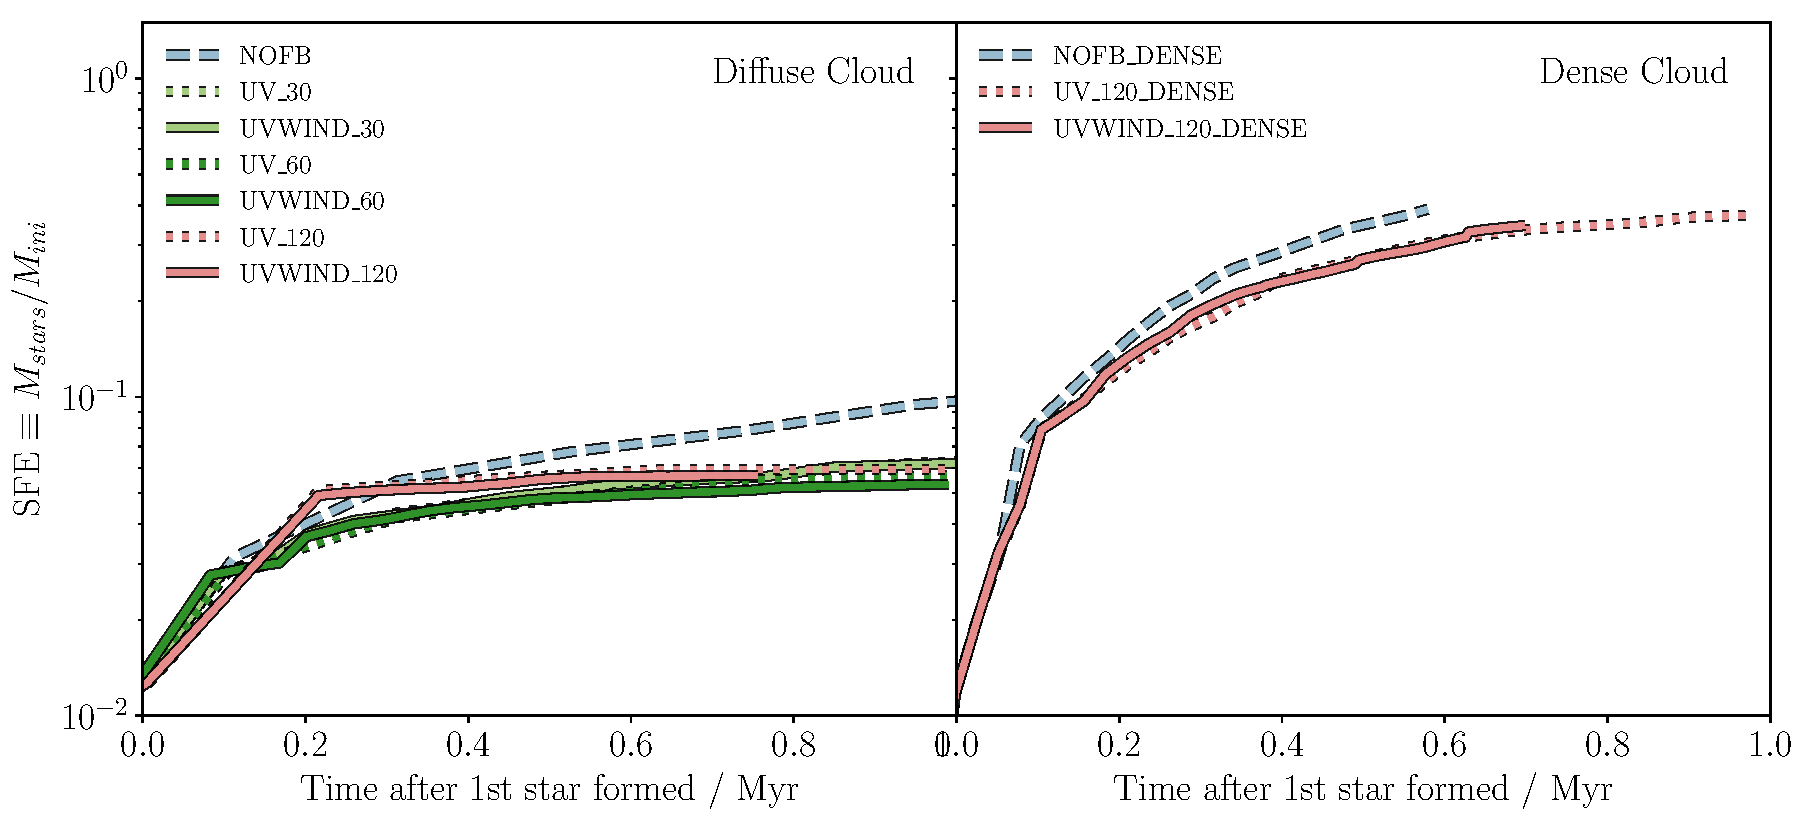
\includegraphics[width=2\columnwidth]{../plots/tsfe_both.pdf}
	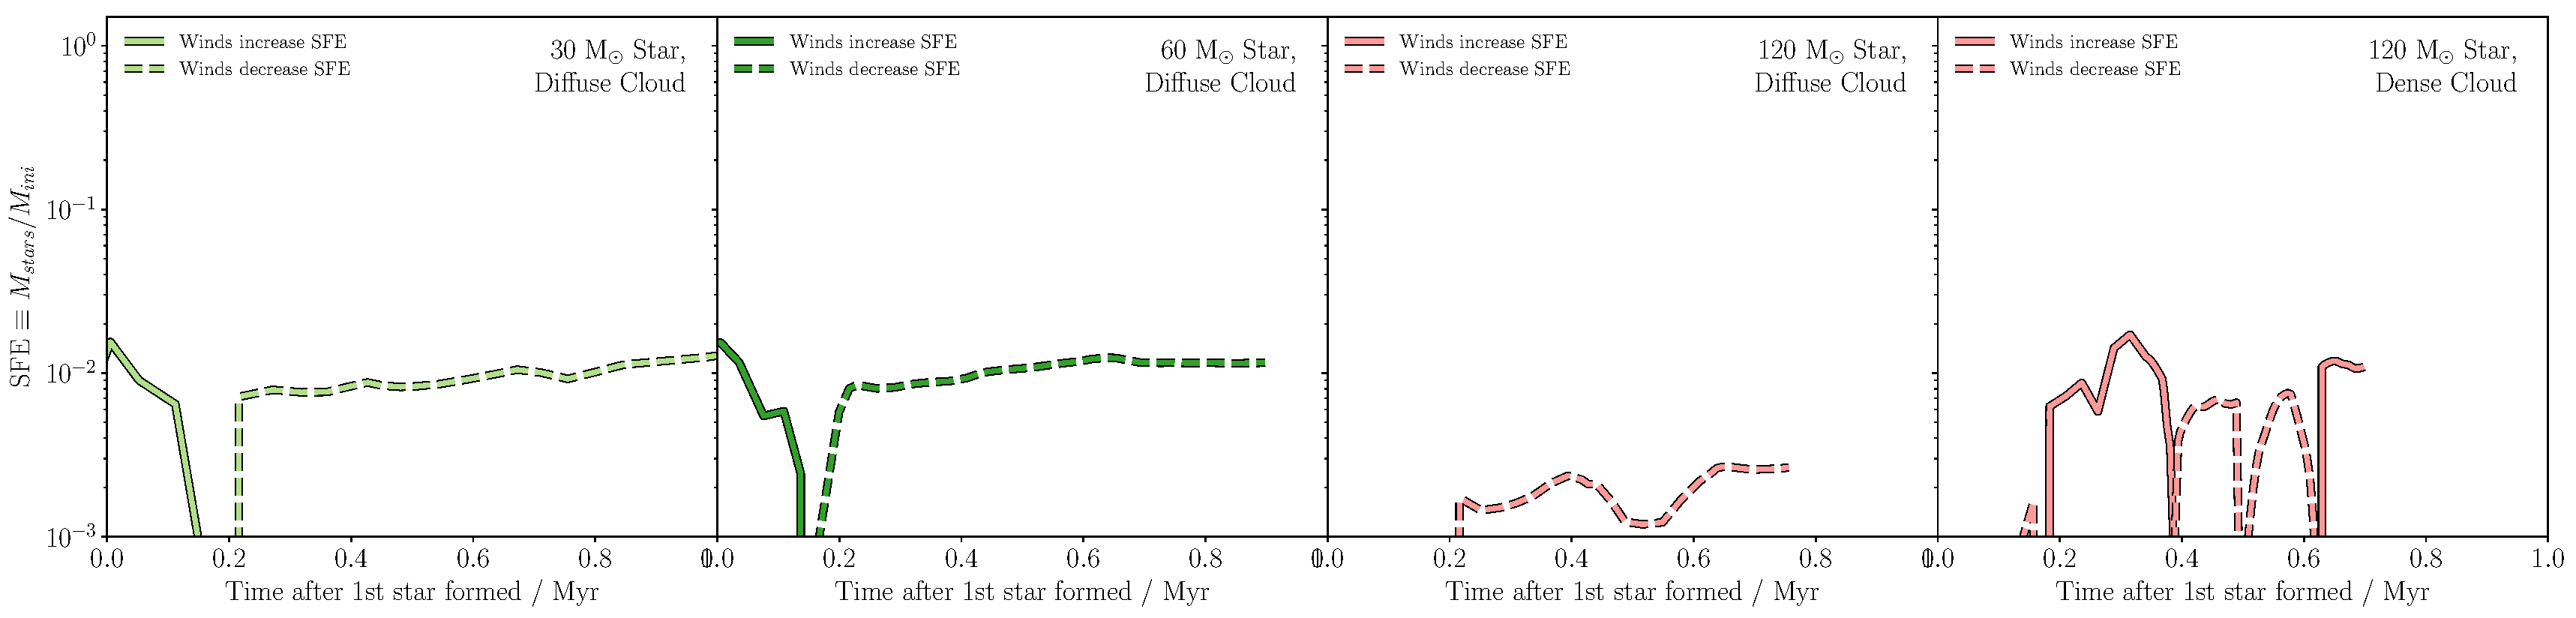
\includegraphics[width=2\columnwidth]{../plots/tsfe_both_compare.pdf}
	\caption{Fraction of total initial cloud mass turned into stars in each simulation, representing the Star Formation Efficiency (SFE). As in Figure \ref{fig:radius}, the upper panels show the absolute SFE and the bottom panels show the difference between the SFE in simulations containing UV photoionisation with and without winds.  A solid line means adding winds gives a larger SFE, a dashed line means adding winds gives a smaller SFE.}
	\label{fig:tsfe}
\end{figure*}

In Figure \ref{fig:tsfe} we plot the fraction of gas initially in the cloud accreted onto sink particles, which we interpret as a measure of \SFE. In the absence of forms of feedback the \SFE grows towards 1. When feedback is included after some early time this figure saturates at a lower value as \HII regions around the first stars formed in the cloud evaporate and disperse dense star-forming gas. We discuss the role of \IMF sampling and cloud structure in setting exactly which value the SFE saturates at in \cite{Geen2018}.

Winds do not as effectively prevent gas from forming stars. Due to this fact and the fact that wind simulations are up to 100 times more costly in terms of computational resources than simulations with just UV photoionisation, we stop the wind simulations when the simulations containing just UV photoionisation saturate their \SFE.

The simulations containing UV photoionisation with and without wind show similar results. In the M4 ($10^4$ \Msolar) cloud, there is a negligible difference. The differences peak at $\pm$0.003 compared to a total SFE of 0.05, most of which appear to be statistical variations rather than a systemic trend.

In the M5 ($10^5$ \Msolar) cloud, there is a systemic increase of 0.01 in SFE compared to a total SFE of 0.2. This figure drops over time. This suggests that there is a small triggering of star formation from the addition of stellar winds, but also that much of the triggering appears to be temporary. Based on the proposals of \cite{Dale2015}, we suggest that this effect is caused by the temporary acceleration of star formation in structures that would form stars anyway, rather than the triggering of new star formation in otherwise stable gas. This does not happen in the M4 cloud for one of two reasons: 1) there are fewer colliding flows since there are fewer spatially-separated star-forming structures, or 2) the shorter freefall time of the M5 cloud causes more rapid fragmentation than in the M4 cloud. A full analysis of this effect is complex and beyond the scope of this paper.

\subsection{Momentum}

\begin{figure*}
	% To include a figure from a file named example.*
	% Allowable file formats are eps or ps if compiling using latex
	% or pdf, png, jpg if compiling using pdflatex
	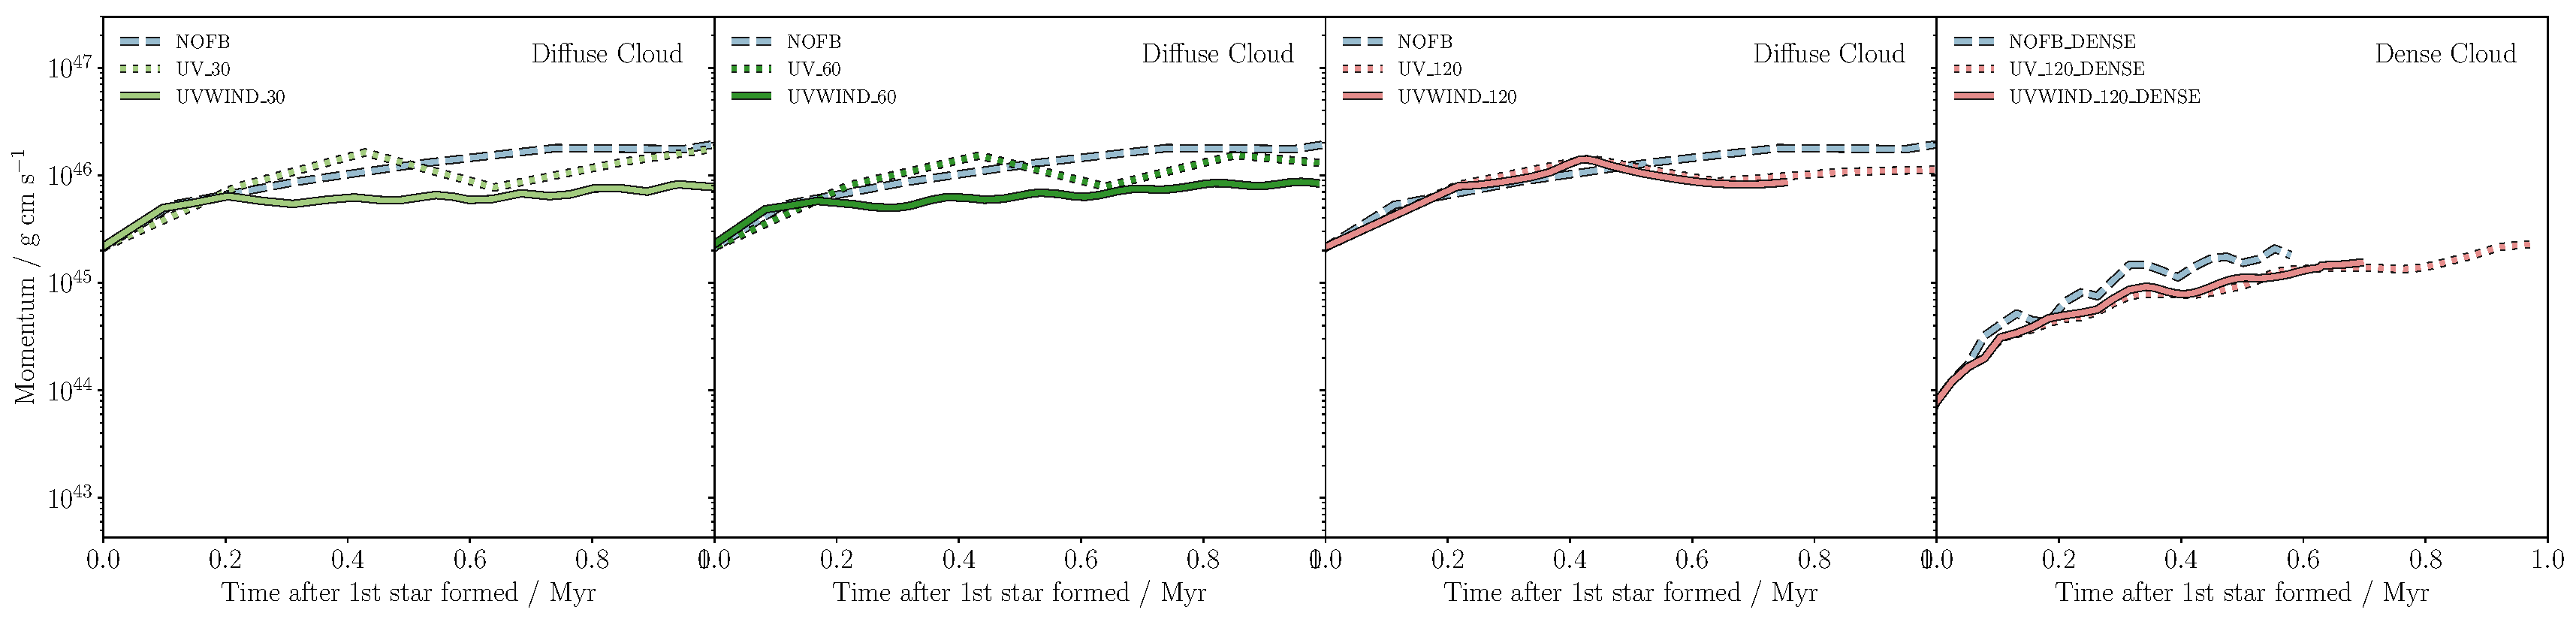
\includegraphics[width=2\columnwidth]{../plots/momentum_both.pdf}
	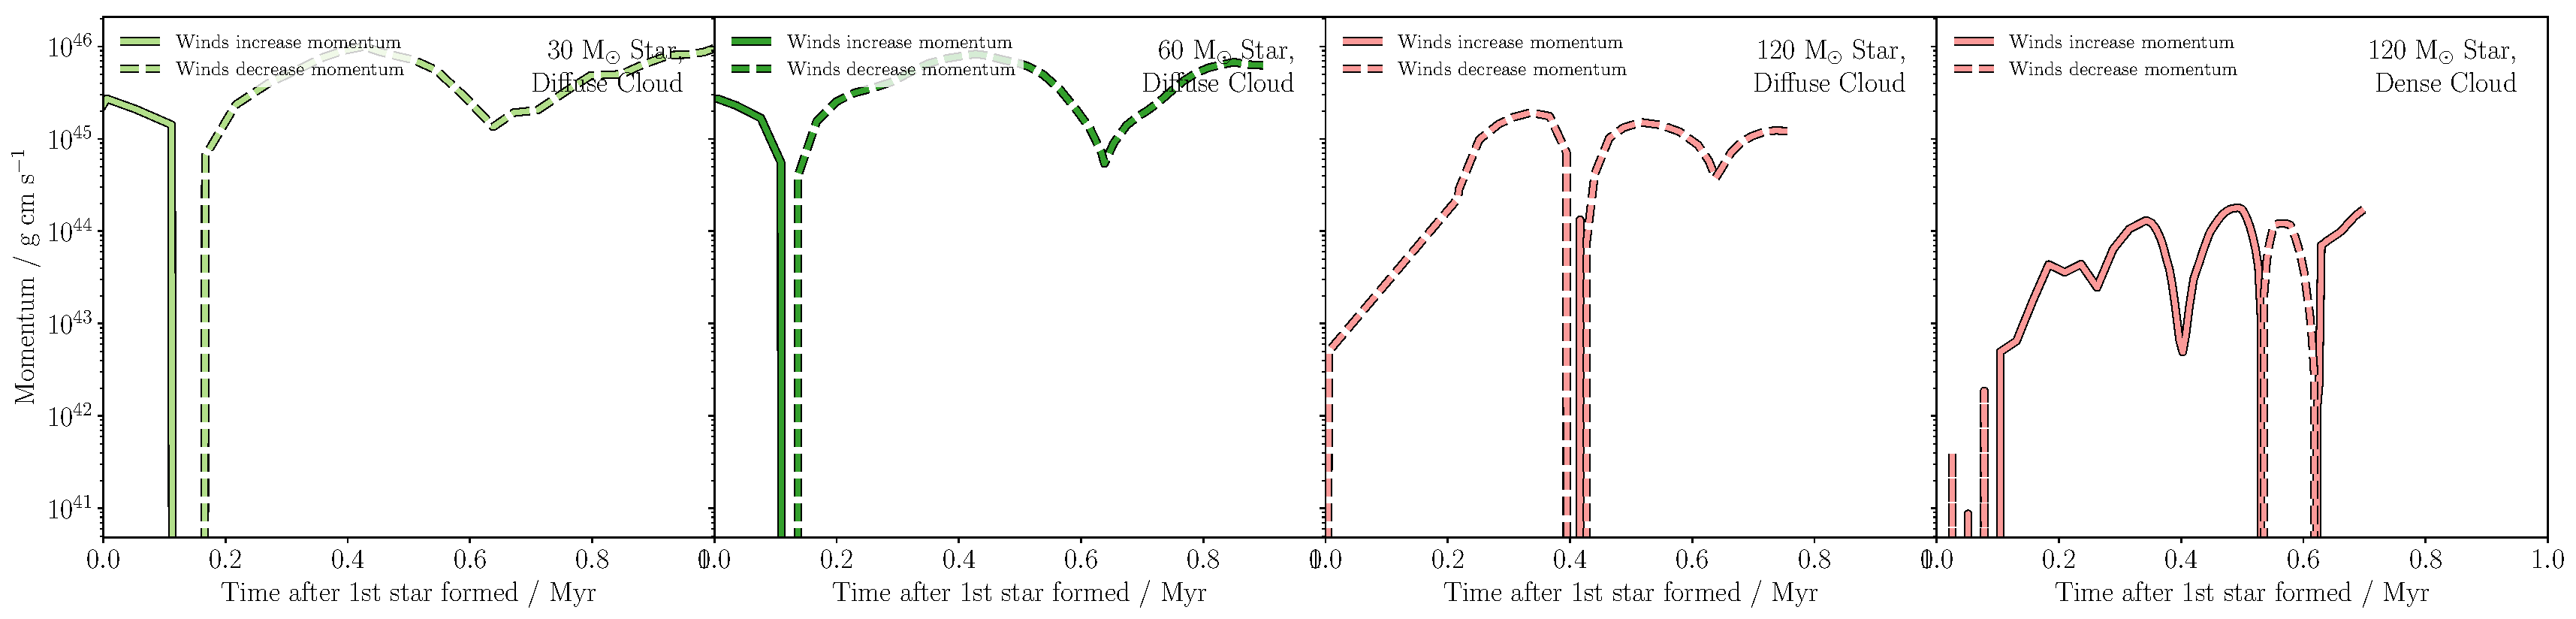
\includegraphics[width=2\columnwidth]{../plots/momentum_both_compare.pdf}
	\caption{Total momentum of the gas in each simulation. As in Figure \ref{fig:radius}, the upper panels show the absolute momentum and the bottom panels show the difference between the momentum in simulations containing UV photoionisation with and without winds.  A solid line means adding winds gives more momentum, a dashed line means adding winds gives less momentum.}
	\label{fig:momentum}
\end{figure*}

REMOVE FIT LINES??? SORT OF DIFFICULT TO FOLLOW, PROBLEMS WITH NORMALISATION OF t=0
MAKE LINEAR TIME IN ALL FIGURES

In Figure \ref{fig:momentum} we measure the total momentum in all gas flows in the simulation volume in all directions. The initial momentum in the box is the momentum of turbulent flows in the cloud prior to the formation of the first \HII region. The initial momentum in the M5 cloud is over 10$\times$ the momentum in the M4 cloud since its freefall time is shorter, and so the escape velocity is higher. The time taken for the momentum of the \HII region(s) to exceed this background is also longer. 

As with the \SFE, the contribution of UV photoionisation to the momentum of the \HII region is larger than the contribution from stellar winds in all cases. After around 2 Myr in each simulation, flows begin to leave the box and we lose the ability to track the momentum of this material. This is consistent with the argument by \cite{Franco1990} and others that the speed of the ionisation front in an isothermal cloud should be around 3 times the speed of sound in the ionised gas, or approximately 30 km/s. 

Since we do not track larger scale flows outside the cloud, the momentum of material that has left the cloud will in any case be affected by external flows - for example, \cite{Cioffi1988} argue that after a certain time, momentum from supernova remnants should merge with the background turbulence. As in \cite{Haid2018}, the external medium should also be ionised from external sources, reducing the impact of ionising photons on material outside the cloud.

Comparing the momentum in UV photoionisation simulations with and without winds, we can argue that winds contribute up to 10\% of the momentum in all cases after a few hundreds kyr, before which they have no effect or even reduce the total momentum from flows.

In the first 0.1 to 0.3 Myr, including winds does not boost the momentum deposited of the \HII region. In fact, in the M5 cloud they even appear to reduce it. This effect is particularly visible in the M5 cloud results. In GEEN2018B we show that winds should have a larger impact on the expansion of the \HII region since the small initial radius gives a smaller surface area over which the wind energy is deposited. While this does not trap the ionising radiation particularly efficiently in our simulations, it will modify the early evolution of the \HII region. A small dense shell around the wind bubble will increase the recombination rate for a parcel of gas, reducing the ability for UV photons to ionise more gas. As the shell is depleted and the wind bubble expands, the effect of winds becomes to create a collisionally-ionised volume that does not need to be photoionised, causing the ionisation front to travel further.

An alternative explanation, however, is that at early times the signal from feedback is weaker than the background turbulence of the cloud, and it takes time for the signal from feedback to grow to the point where it is significant. More careful controlled tests are needed to confirm which of these hypotheses is correct.


\subsection{\HII Region Expansion}

\begin{figure*}
	% To include a figure from a file named example.*
	% Allowable file formats are eps or ps if compiling using latex
	% or pdf, png, jpg if compiling using pdflatex
	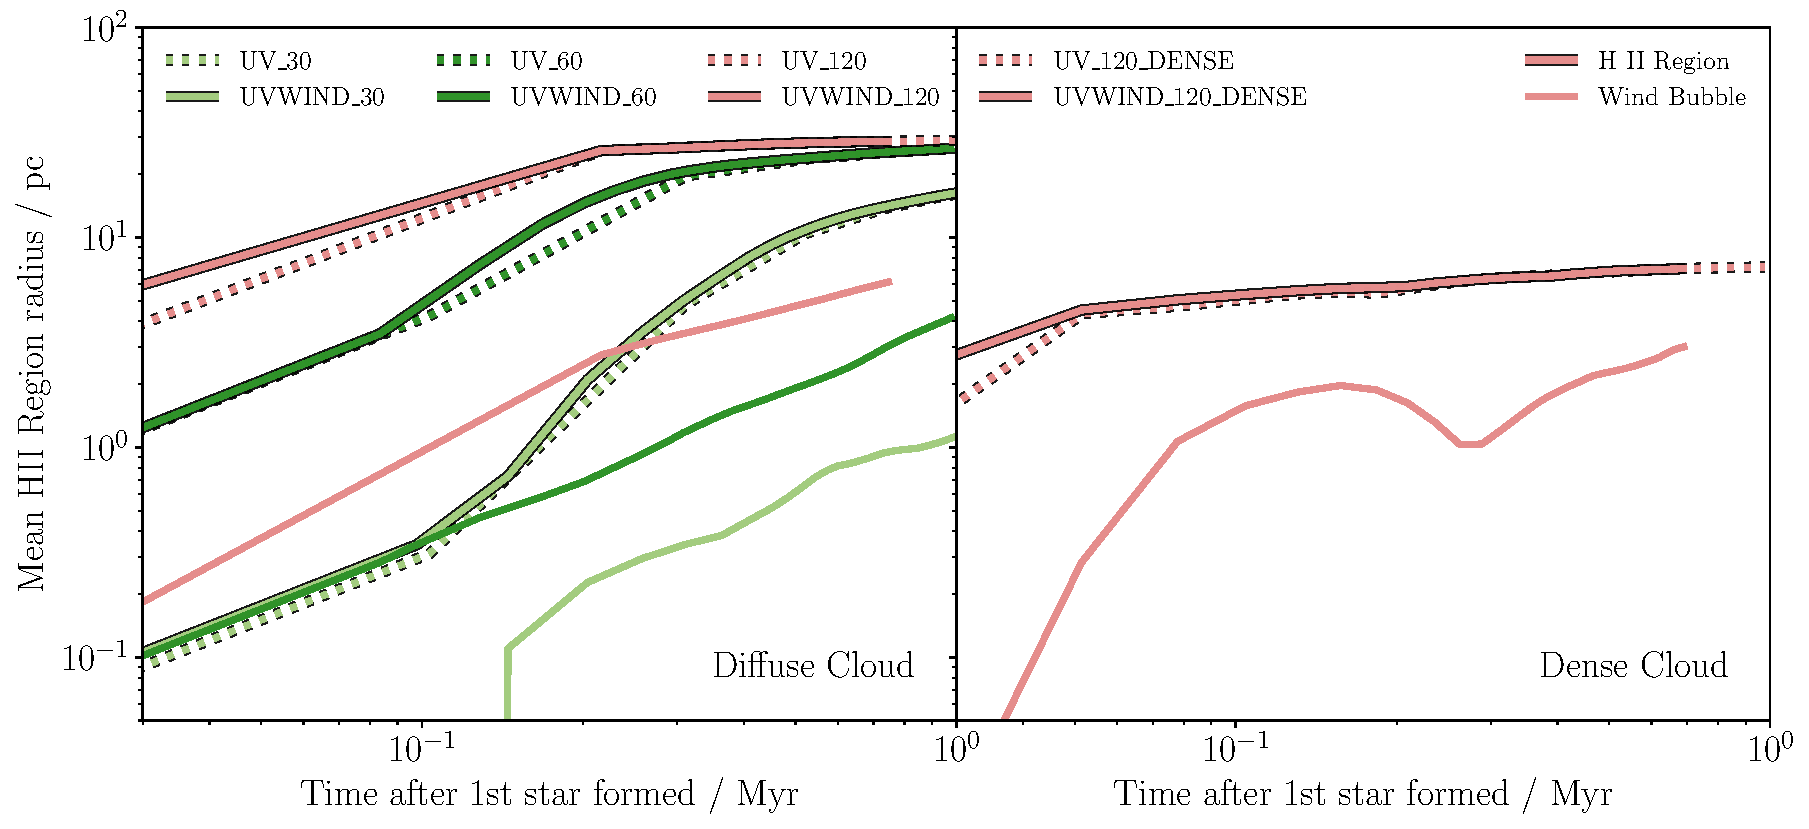
\includegraphics[width=2\columnwidth]{../plots/radius_both.pdf}
	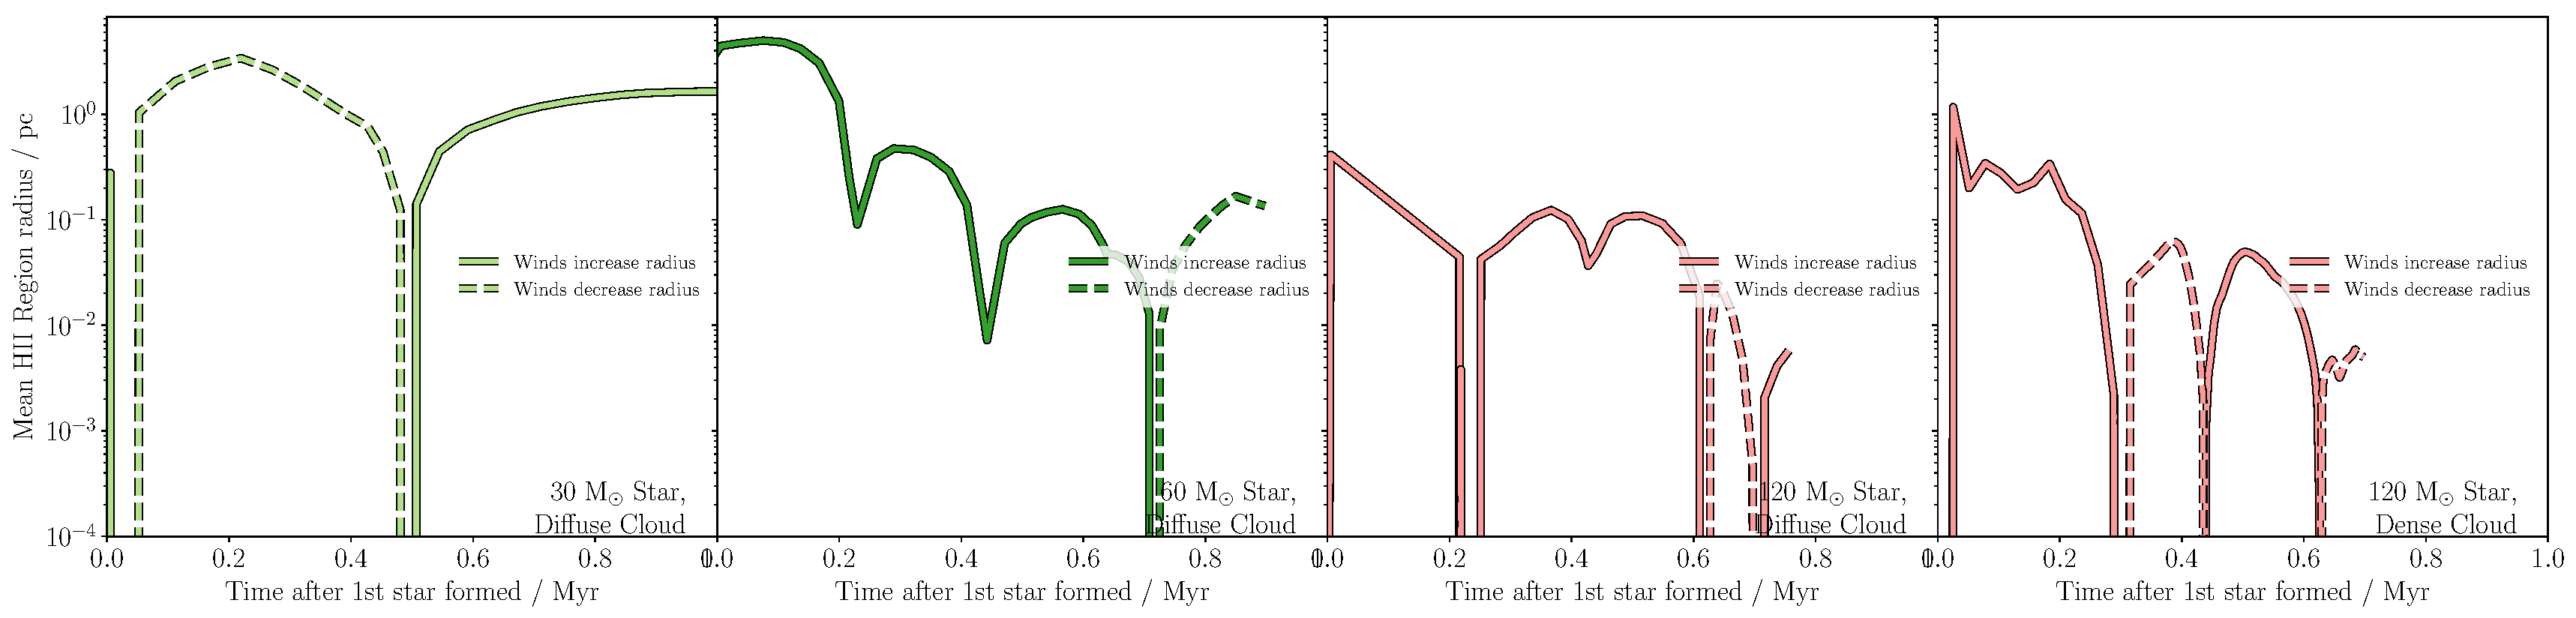
\includegraphics[width=2\columnwidth]{../plots/radius_both_compare.pdf}
	\caption{Sphericised total radius of the \HII regions in each simulation. This is calculated by finding the volume of all cells above $x_{\HII}>0.1$ and then calculating $(3 V /4 \pi)^{1/3}$ for these cells where $V$ is their volume. The upper panels show the absolute sphericised radius, while the lower panels show the difference between the radius in simulations containing UV photoionisation with and without winds. A solid line means adding winds gives a larger radius, a dashed line means adding winds gives a smaller radius.}
	\label{fig:radius}
\end{figure*}

\begin{figure*}
% To include a figure from a file named example.*
% Allowable file formats are eps or ps if compiling using latex
% or pdf, png, jpg if compiling using pdflatex
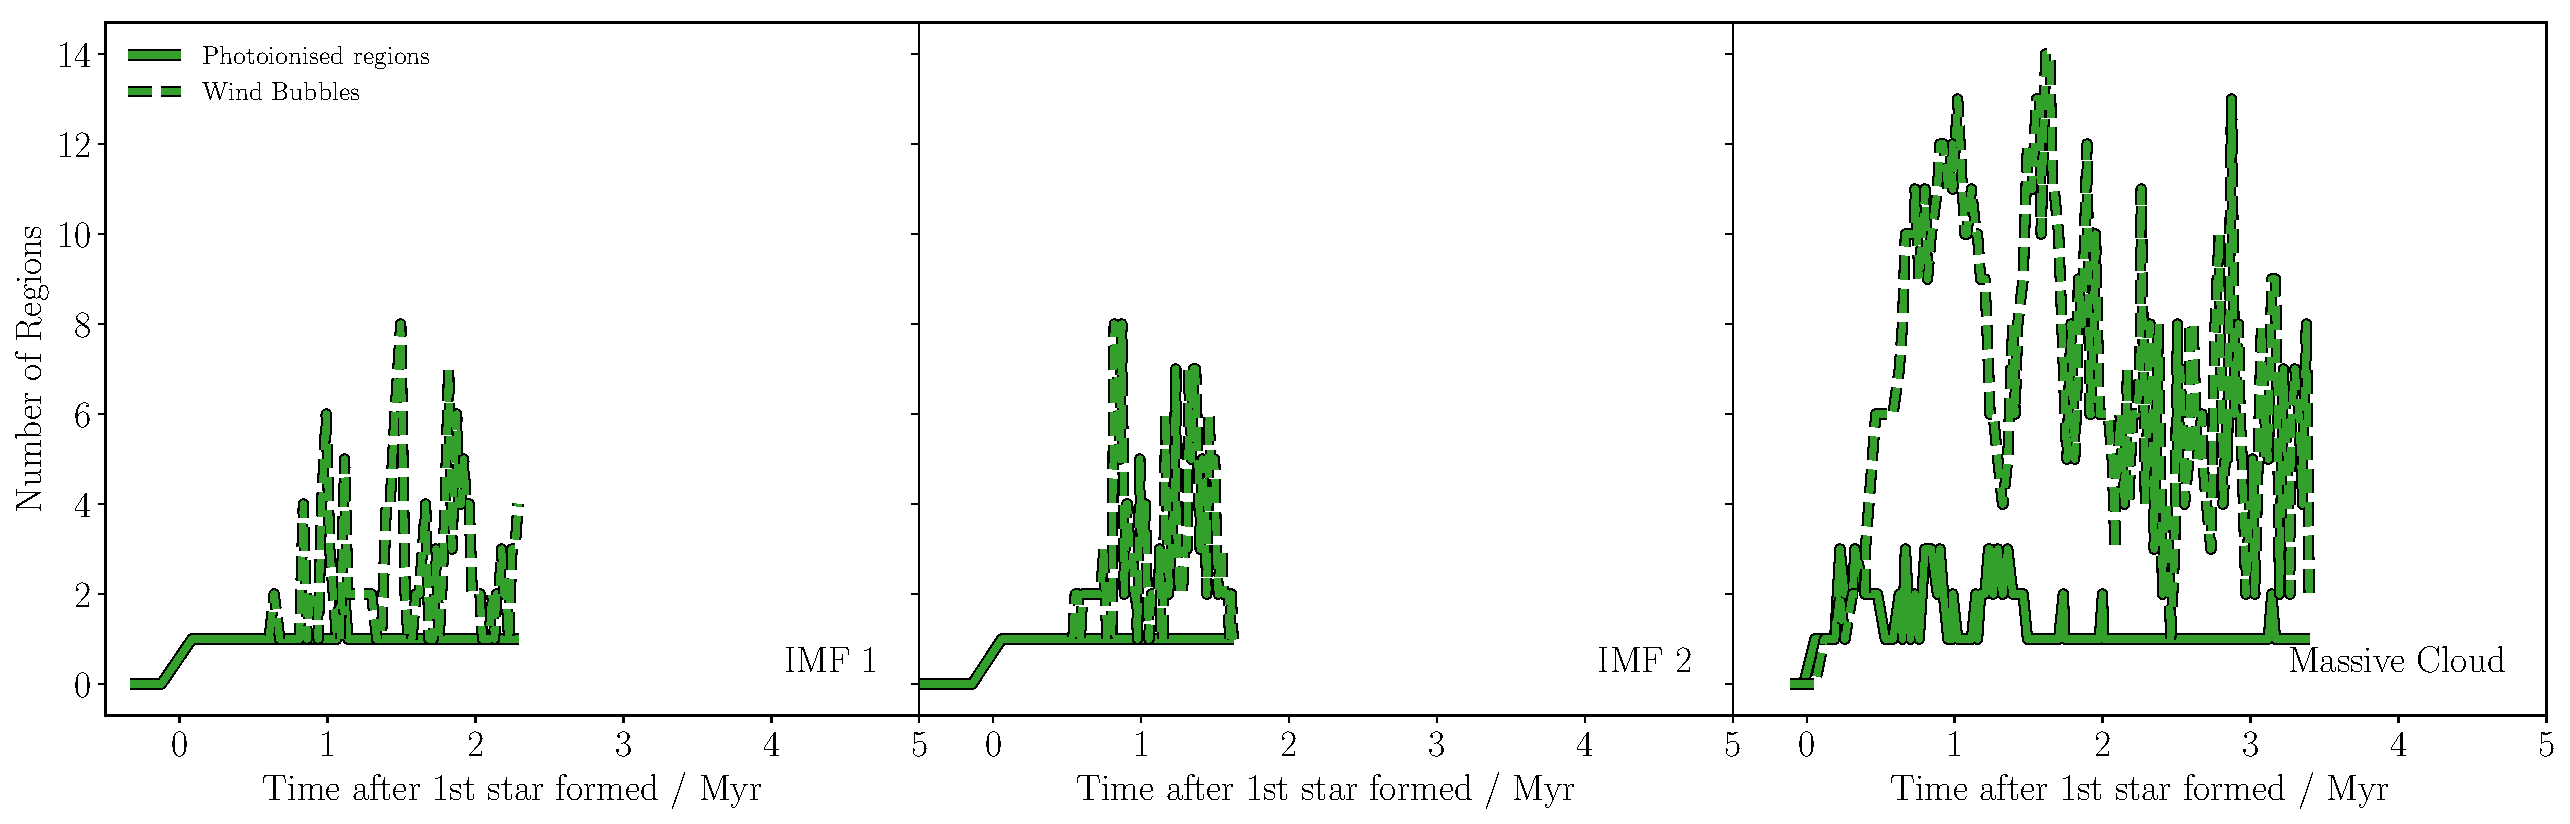
\includegraphics[width=2\columnwidth]{../plots/findHIIregions.pdf}
\caption{Number of \HII regions and stellar wind bubbles in runs containing both UV photoionisation and stellar winds. \HII regions are identified as contiguous volumes where $x_{\HII} > 0.1$. Wind bubbles are defined as contiguous volumes where either the temperature is above $10^5$ K or the speed of the gas is above 500 km/s (or both). The noisiness of the wind bubble results may indicate flaring and separation of hot bubbles from the stellar source as well as multiplicity of sources.}
\label{fig:HIIregions}
\end{figure*}

RADIUS PEAKS IN IMF2 BECAUSE IT LEAVES THE BOX VERY EARLY

As with the other parameters, UV photoionisation is the principal driver of the photoionisation regions as shown in Figure \ref{fig:radius}. The radial expansion is rapid as the ionisation front leaves the isothermal cloud profile, then slows as it hits the uniform external medium.

The winds add approximately 1 pc to the \HII region radius when the DIM IMF is used, and up to 5-6 pc when the BRIGHT IMF is used. We return to this result in Section \ref{analytic_comparison}.

The M5 cloud has less smooth radial expansion than the M4 cloud. This is because the cloud contains multiple independent \HII regions at various times. In Figure \ref{fig:HIIregions} we plot the number of independent photoionised \HII regions and wind bubbles at each time. Wind bubbles in this case are defined as gas above either $10^5$ K or travelling faster than 500 km/s.

In the M4 cloud, there is typically only one contiguous photoionised \HII region, with the exception of one output at 4.5 Myr in M4-DIM-UV+WIND. In the M5 cloud, for roughly 3 Myr there are 2 or even 3 regions that form and eventually merge into the larger region.

The number of wind bubbles behaves more erratically. In the M4 cloud these spike at anywhere between 1 and 8 distinct bubbles, before the bubbles disappear or merge into a single wind bubble. In the M5 cloud, there are up to 14 distinct regions at any one time, with multiple independent regions persisting for multiple Myr. This reduces the combined effect of winds, as described by \cite{Silich2017}, since each massive star creates its own small wind bubble rather than contributing to a single bubble. We return to this argument in Section \ref{analytic_comparison}.

\section{Analytic Comparison}
\label{analytic_comparison}

In GEEN2018B, we track the evolution of photoionised \HII regions containing stellar winds and radiation pressure through isothermal power law density fields. We define these as density profiles $n(r) = n_0 (r / r_0)^{-w}$, where $w=2$. 

In this Section we evaluate the effects of stellar winds on more physically complete simulations of \HII regions in complex environments with self-consistent star formation. A fully rigorous analysis is difficult due to the complexity of the 3D system, so we limit ourselves to the broad predictions made by the analytic results and leave a more exhaustive comparison to future simulation work in more idealised conditions.

\subsection{Cloud Properties at First Star Formation}
\label{ana:cloudprops}

\begin{figure*}
% To include a figure from a file named example.*
% Allowable file formats are eps or ps if compiling using latex
% or pdf, png, jpg if compiling using pdflatex
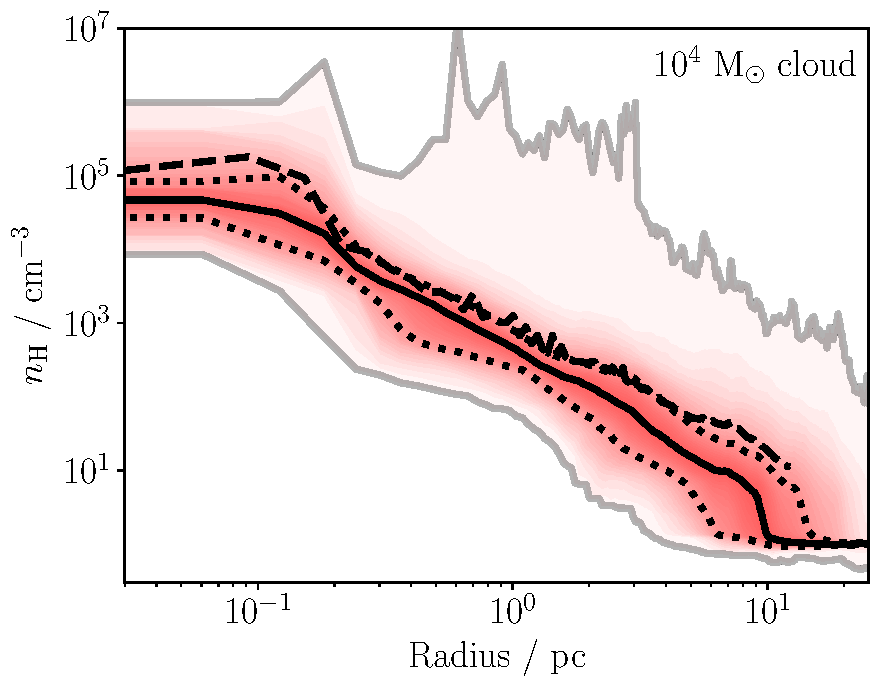
\includegraphics[width=\columnwidth]{../plots/gradrays/IMF1_01/nH/profile_starpos00018.pdf}
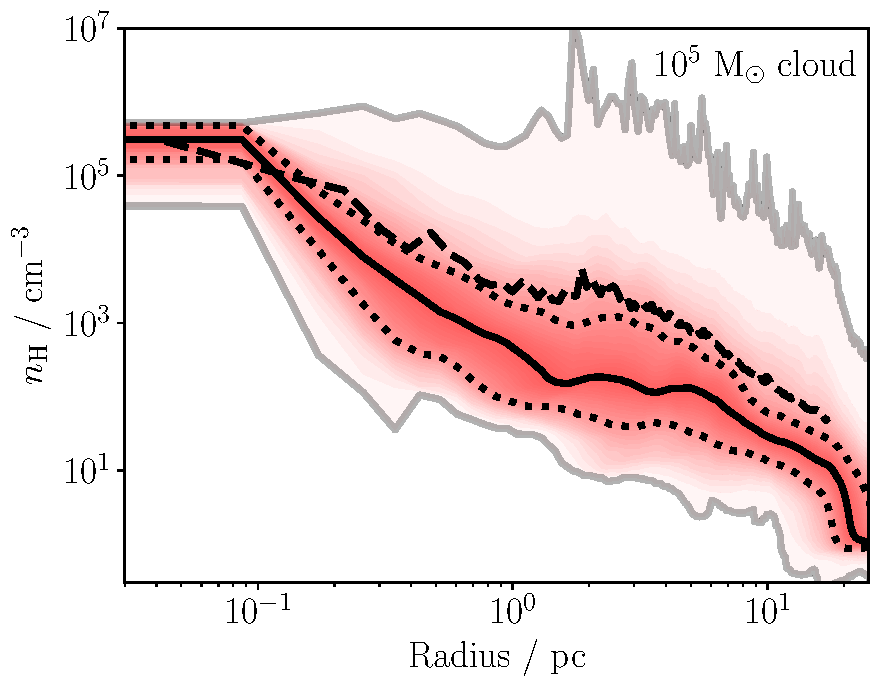
\includegraphics[width=\columnwidth]{../plots/gradrays/MASS_01/nH/profile_starpos00016.pdf}
\caption{Probability distribution functions for volume density in each cloud around the first star formed in the simulation at the time of its formation. The plot on the left shows simulation M4-NOFB at 3.38 Myr after the start of the simulation, while the plot on the right shows M5-NOFB at 1.2 Myr. In each plot we draw rays from the star out to half a box length and calculate statistics for the density field at each radius for each ray. The black solid line shows the median profile (i.e. the value for which 50\% of the densities at a given radius lie above), while the dashed line shows the mean profile. The dotted lines show the interquartile range, while the grey lines show the maximum and minimum. The red shading shows the linear probability, with deeper red being closer to the median. Below $\sim$0.1 pc the density field is affected by accretion onto the sink particle.}
\label{fig:gradrays}
\end{figure*}

\begin{figure}
	% To include a figure from a file named example.*
	% Allowable file formats are eps or ps if compiling using latex
	% or pdf, png, jpg if compiling using pdflatex
	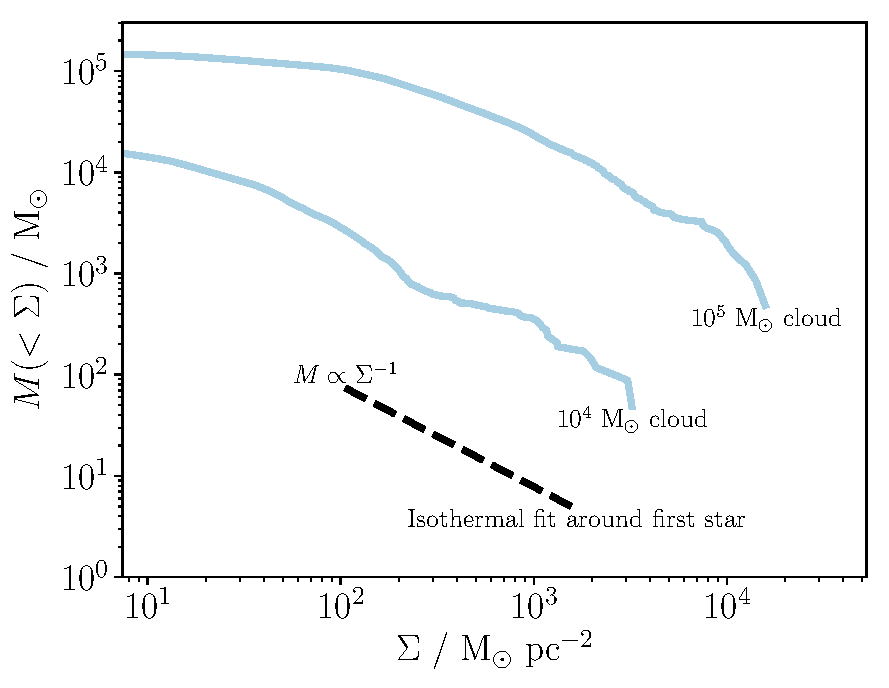
\includegraphics[width=\columnwidth]{../plots/cumuldens.pdf}
	\caption{Mass inside contours defined by a given surface density $\Sigma$ at the time of first star formation in each cloud. The upper blue line shows the M5-NOFB simulation at 1.2 Myr, while the lower blue line shows the M4-NOFB simulation at 3.38 Myr. Overplotted is the fit for an isothermal profile with the values given in Equation \ref{ana:nr_M4} at $r < 1$ pc.}
	\label{fig:cumuldens}
\end{figure}

In Figure \ref{fig:gradrays} we plot the probability distribution functions for cloud density at each radial bin around the first star to form in the simulations. The radius under 0.1 pc is mostly set by the sink particle accretion radius, since the smallest cell size is 0.03 pc in the M4 cloud and 0.04 pc in the M5 cloud.

Above 0.1 pc, the M4 ($10^4$ \Msolar) cloud has a median density profile that is roughly isothermal. The M5 ($10^4$ \Msolar) cloud has an isothermal profile up to $\sim$1 pc, where other dense clumps flatten the profile. Specifically, we find for cloud M4:
\begin{equation}
\begin{split}
n(r) = 432~\mathrm{cm}^{-3} (r / 1~\mathrm{pc})^{-1.98}~\mathrm{for}~ 0.1 < r/\mathrm{pc}< 1 \\
n(r) = 3.74~\mathrm{cm}^{-3} (r / 10~\mathrm{pc})^{-2.10}~\mathrm{for}~ 0.1 < r/\mathrm{pc}< 10 \\
\end{split}
\label{ana:nr_M4}
\end{equation}
which is relatively consistent for both parts. We use $r_0$ as the outer limit for the density distribution sampled as in GEEN2018B, since we are interested in the state of the \HII region at this point.

In the M5 cloud, we find 
\begin{equation}
\begin{split}
n(r) = 390~\mathrm{cm}^{-3} (r / 1~\mathrm{pc})^{-2.26}~\mathrm{for}~ 0.1 < r/\mathrm{pc}< 1 \\
n(r) = 37.4~\mathrm{cm}^{-3} (r / 10~\mathrm{pc})^{-1.21}~\mathrm{for}~ 0.1 < r/\mathrm{pc}< 10 \\
\end{split}
\label{ana:nr_M5}
\end{equation}

Both clouds thus have profiles inside $r_0=1$ pc where $n_0\simeq400$ cm$^{-3}$ and $w\simeq-2$, with a slightly steeper profile in the M5 cloud. The profiles become more different at larger radii due to the presence of other dense structures, with a flatter outer profile in the M5 cloud since there are more structures in this cloud. We thus expect the first \HII region to behave similarly up to 1 pc radius, then evolve differently as it envelopes the rest of the cloud and encounters other \HII regions. Note that this is not an exhaustive survey, and the conditions in any case will evolve with time and as other \HII regions begin to evaporate star-forming clumps.

One additional interpretation is that the M5 cloud returns to an isothermal profile after 5 pc until it hits the external medium at 20 pc. Fitting inside this range gives
\begin{equation}
\begin{split}
n(r) = 32.1~\mathrm{cm}^{-3} (r / 10~\mathrm{pc})^{-2.04}~\mathrm{for}~ 5 < r/\mathrm{pc}< 20 \\
\end{split}
\label{ana:nr_M5_20pc}
\end{equation}
which is roughly a factor of 10 denser than the M4 cloud's profile. We return to this interpretation in Section \ref{ana:HIIregioniso}.

The median density at each radius (the solid line in Figure \ref{fig:gradrays}) is lower than the mean density since it is less affected by dense clumps, which contain a lot of mass but have relatively lower angular size from the point of view of the first star. In this context, the typical profile that an outflow leaving the star ``sees'' is the median profile. We therefore use this profile, and not the mean profile, for the analysis in this paper. The mean profile is typically flatter due to the effect of other dense clumps that increase in frequency with the volume of radial elements. In this paper we typically find power law profiles with index $w\simeq-2$, whereas in \cite{Geen2018} where we measure the mean profile, $w \simeq 1.7$.

In Figure \ref{fig:cumuldens} we plot the mass inside contours defined by a given surface density $\Sigma$ at the same times as Figure \ref{fig:gradrays}. In a single isothermal profile where $w=-2$, 
\begin{equation}
M(<\Sigma) = (2 \pi n_0 r_0^2 m_H / X)^2 / \Sigma.
\label{ana:MvsSigma}
\end{equation}
A cloud defined by a set of multiple independent profiles matching this description will also have a similar dependence, with the resulting mass simply being the sum of the result for each profile. We overplot the Equation \ref{ana:MvsSigma} for the values given in Equation \ref{ana:nr_M4} in the fit at $r < 1$ pc.

The slope of both clouds is consistent with the hypothesis that the cloud is composed of a set of isothermal profiles distributed across the cloud volume. At high densities the profile breaks down since the simulations reach their maximum spatial resolution and sink particles begin accreting the extra mass. At low densities, the profiles hit the edge of the cloud and the external volume becomes uniform. We should caution that the overall picture is likely more complicated than a neat set of spherical profiles overlaid in a fixed volume. However, it is a useful picture from which to begin understanding the evolution of \HII regions within this set of structures.

\subsection{Evolution of H II Regions in Isothermal Profiles}
\label{ana:HIIregioniso}

% Clouds
\begin{table}
	\centering
	\caption{List of coefficients indicating the effect of winds ($C_w$), radiation pressure from ionising photons ($C_{rp}$) and gravity ($C_{grav}$) on the \HII region at the 100 \Msolar surface density contour (see Figure \protect\ref{fig:cumuldens}). A value larger than 1 (in bold face) indicates that the effect has a larger contribution to the \HII region than UV photoionisation, and a much smaller value indicates negligible dynamic influence on the radius and structure of the \HII region. As stated in Section \protect\ref{methods}, the DIM IMF sampling produces fewer photons at early times than BRIGHT, since it starts with a lower mass star (31 \Msolar versus 68 \Msolar).}
	\label{ana:CwCrpCg}
	\begin{tabular}{cccccccc} % four columns, alignment for each
		\textbf{Cloud Mass}    & \textbf{Cluster} & $C_w$    & $C_{rp}$ & $C_{grav}$ \\
		\hline
		\multicolumn{4}{l}{Whole cloud, $\Sigma = 10^2$ \protect\Msolarpc} \\
		\hline
		$10^4$ \Msolar  & DIM     & 0.0037 & 0.31     & 0.14       \\
		$10^4$ \Msolar  & BRIGHT  & 0.040  & 0.46     & 0.14       \\
		$10^5$ \Msolar  & BRIGHT  & 0.043  & \textbf{33}       & 0.32       \\
		\hline
		\multicolumn{4}{l}{Whole cloud, $\Sigma = 10^3$ \protect\Msolarpc} \\
		\hline
		$10^4$ \Msolar  & DIM     & 0.128  & 0.933    & 0.20       \\
		$10^4$ \Msolar  & BRIGHT  & \textbf{1.4}    & \textbf{1.4}      & 0.20       \\
		$10^5$ \Msolar  & BRIGHT  & 0.53   & \textbf{84}       & 0.46       \\
		\hline
		\multicolumn{4}{l}{First \protect\HII region at 1 pc (Equations \protect\ref{ana:nr_M4}, \protect\ref{ana:nr_M5})} \\
		\hline
		$10^4$ \Msolar  & DIM     & 0.0048 & 0.096    & 0.056      \\
		$10^4$ \Msolar  & BRIGHT  & 0.088  & 0.27     & 0.056      \\
		$10^5$ \Msolar  & BRIGHT  & 0.086  & 0.27     & 0.052      \\
		\hline
		\multicolumn{4}{l}{First \protect\HII region at 10 pc (Equation \protect\ref{ana:nr_M5_20pc} in M5 cloud only)} \\
		\hline
		$10^5$ \Msolar  & BRIGHT  & 0.010  & 0.086     & 0.14      \\
		
	\end{tabular}
\end{table}

In GEEN2018B we solve for the evolution of a D-type photoionisation front inside an isothermal density profile. We include the influence of gravity and external accretion, winds and radiation pressure. We treat winds as a collisionally-ionised bubble inside the \HII region that due to its fast sound speed ($\sim$1000 km/s versus $\sim$10 km/s in the photoionised gas) is in hydrostatic equilibrium with the photoionised gas. In the paper we calculate limits where gravity, winds and radiation pressure are likely to significantly alter the evolution of the \HII region.

As shown in the previous section, the M4 cloud can be treated as a roughly single isothermal sphere as described in Equation \ref{ana:nr_M4}. While the cloud's mass distribution suggests the presence of many isothermal profiles distributed around the same volume, the median density profile (i.e. the typical path seen by a photon travelling from the star to the edge of the cloud) remains roughly on the same power law density profile.

The M5 cloud is more complex. The inner parsec of both clouds around the first star formed has a very similar isothermal profile. After 1 pc in the M5 cloud, the profile flattens out, before becoming isothermal again at 5 pc until the edge of the cloud at 20 pc. We posit that the higher mass of the structure leads to more dense structures existing inside the same cloud, whose distribution modifies the average profile.

NOTES

RADIATION PRESSURE IS COOL AT THE EDGE OF THE CLOUD BUT DOESN'T DO MUCH IN THE FIRST HII REGION
SO WE MIGHT SEE LARGE EMPTY HII REGIONS BUT THEY DON'T DO MUCH ON SMALLER SCALES
ALSO SOUND SPEED LIMITS ABILITY FOR RADIATION PRESSURE TO COMPLETELY EVACUATE THE BUBBLE??
EFFECT OF WINDS OVERSTATED BECAUSE THEY'RE IN INDIVIDUAL BUBBLES
MASS INSIDE SIGMA INCLUDES ALL CLUMPS, MEAN DENSITY ~ 0.1-0.2 DEX ABOVE MEDIAN -- DENSER MATERIAL TO PUSH OUT, ESPECIALLY IN MASSIVE CLOUD
SOLVE COEFFICIENTS FOR THE MASSIVE CLOUD OUTER MEDIAN PROFILE
MENTION ASSUMPTIONS FOR F(T)

\section{Discussion}

DISCUSSION

\section{Conclusions}

CONCLUSIONS

\section*{Acknowledgements}

ACKNOWLEDGEMENTS
Jo Puls

The authors gratefully acknowledge the data storage service SDS@hd supported by the Ministry of Science, Research and the Arts Baden-W\"urttemberg (MWK) and the German Research Foundation (DFG) through grant INST 35/1314-1 FUGG.

%%%%%%%%%%%%%%%%%%%%%%%%%%%%%%%%%%%%%%%%%%%%%%%%%%

%%%%%%%%%%%%%%%%%%%% REFERENCES %%%%%%%%%%%%%%%%%%

% The best way to enter references is to use BibTeX:

\bibliographystyle{mnras}
\bibliography{samgeen} % if your bibtex file is called example.bib

%%%%%%%%%%%%%%%%%%%%%%%%%%%%%%%%%%%%%%%%%%%%%%%%%%

%%%%%%%%%%%%%%%%% APPENDICES %%%%%%%%%%%%%%%%%%%%%

\appendix
%
%\section{Appendix Blah}
%
%APPENDIX

%%%%%%%%%%%%%%%%%%%%%%%%%%%%%%%%%%%%%%%%%%%%%%%%%%


% Don't change these lines
\bsp	% typesetting comment
\label{lastpage}
\end{document}

% End of mnras_template.tex